\section{Apache Flink}

\subsection{Overview}

Apache Flink originated as the \emph{Stratosphere} research project at TU Berlin in 2010
and was donated to the Apache Software Foundation in 2014.
Unlike Spark, which added streaming as an extension to a batch engine,
Flink was designed from the ground up as a \textbf{true streaming system}:
batch processing is treated as a special case of streaming over \emph{bounded} data,
rather than the reverse.

\begin{figure}[H]
  \centering
  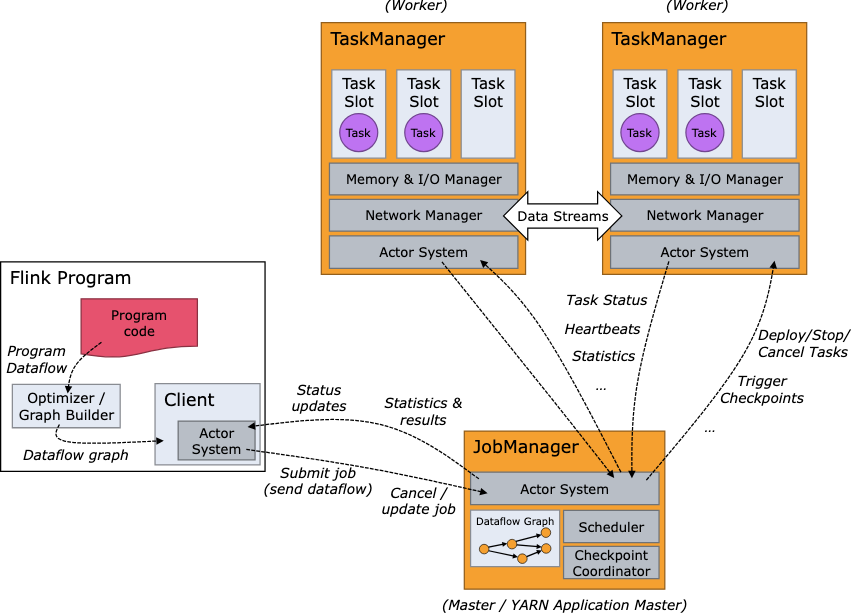
\includegraphics[width=0.88\textwidth]{image/engine/flink_architecture.png}
  \caption{Apache Flink cluster architecture: JobManager, TaskManagers, and the dataflow graph.}
  \label{fig:flink-arch}
\end{figure}

Key runtime components:
\begin{itemize}
  \item \textbf{JobManager} — the cluster master.
        It accepts submitted jobs, translates the user's program into an optimised \emph{execution graph},
        schedules \emph{tasks} (operator instances) onto TaskManagers, coordinates distributed checkpoints,
        and handles failure recovery.
  \item \textbf{TaskManager} — the worker nodes.
        Each TaskManager hosts a fixed number of \emph{task slots} (configurable).
        A task slot runs one parallel pipeline operator; task slots on the same TaskManager can share JVM resources,
        avoiding inter-process communication overhead via \emph{operator chaining}.
  \item \textbf{Dataflow graph} — the execution plan is represented as a directed acyclic graph (DAG)
        of operators connected by \emph{network channels}.
        Data flows record-by-record from source operators through transformation operators to sink operators
        with no artificial batching barrier.
\end{itemize}

\subsection{Flink Streaming}

\begin{figure}[H]
  \centering
  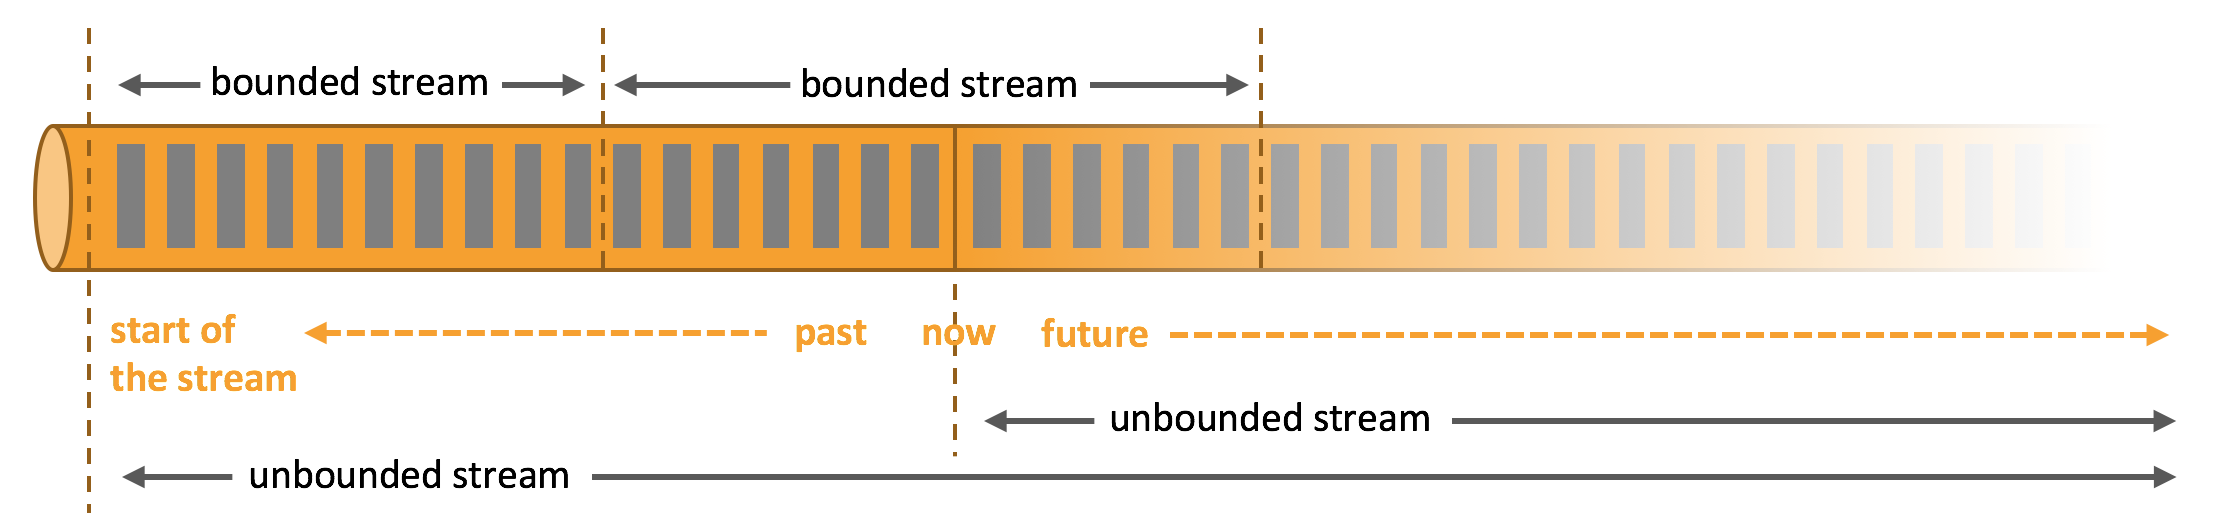
\includegraphics[width=0.88\textwidth]{image/engine/flink_dataflow_unbounded_stream.png}
  \caption{Flink's unbounded stream model: records flow through the operator DAG one event at a time.}
  \label{fig:flink-dataflow}
\end{figure}

Flink processes records \textbf{one event at a time} as they arrive — there is no trigger interval,
no mini-batch accumulation, and no artificial delay.
Results are emitted downstream immediately after each record is processed.

Two programming APIs allow users to work at different levels of abstraction:
\begin{itemize}
  \item \textbf{DataStream API} — a low-level, imperative API that gives full control over operators,
        keyed state, event-time timers, watermark strategies, and process functions.
        Written in Java, Scala, or Python (PyFlink).
  \item \textbf{Table API / Flink SQL} — a high-level, declarative API where the stream is modelled
        as a continuously changing \emph{dynamic table}.
        SQL queries are compiled by the Flink planner into the same dataflow graph as the DataStream API,
        but with significantly less boilerplate.
        This is the API used in the Streamify project (PyFlink Table API + SQL DDL).
\end{itemize}

\subsection{Mechanisms in Flink Streaming}

\subsubsection{How Data is Processed}

Records flow through the operator chain without any buffering barrier:
\begin{enumerate}
  \item The \textbf{Kafka source operator} polls a partition and emits each record immediately downstream.
  \item Intermediate operators (map, filter, join, aggregate) process the record and forward their output
        within the same thread (operator chaining), avoiding serialisation and network hops where possible.
  \item The \textbf{sink operator} writes to the target system (e.g.\ Snowflake via JDBC).
  \item \textbf{Back-pressure} propagates upstream naturally: if a downstream operator is slow,
        its input network buffer fills up, which slows the upstream operator's output, which eventually
        slows the source from polling Kafka — without any explicit rate-limiter or dropped records.
\end{enumerate}

\textbf{Event time and watermarks:}
Flink provides first-class support for \emph{event time} — the timestamp embedded in the record itself,
as opposed to the \emph{processing time} at which the record was received by Flink.
\textbf{Watermarks} are special records injected into the stream at the source that signal
``all events with a timestamp $\leq W$ have now arrived.''
When a windowed operator receives a watermark, it knows it is safe to emit the window result
for all events up to that timestamp, even if some records arrived out of order.
This enables correct window computations (e.g.\ 1-minute tumbling windows) even when records arrive
seconds late due to network delays.

\subsubsection{Checkpointing}

\begin{figure}[H]
  \centering
  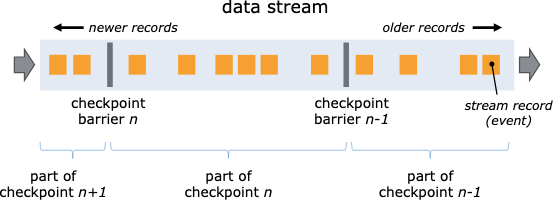
\includegraphics[width=0.88\textwidth]{image/engine/flink_checkpoint.png}
  \caption{Flink distributed snapshot: checkpoint barriers flow through the dataflow graph alongside data records.}
  \label{fig:flink-checkpoint}
\end{figure}

Flink implements fault tolerance via an adaptation of the
\textbf{Chandy-Lamport distributed snapshot algorithm}:

\begin{enumerate}
  \item The JobManager periodically injects \textbf{checkpoint barriers} — special control records —
        into each source partition alongside normal data records.
  \item Each barrier carries a checkpoint ID and flows through the operator graph at the same speed
        as regular records.
  \item When a stateful operator receives barriers from \emph{all} its input channels,
        it takes an \textbf{asynchronous snapshot} of its current state and forwards the barrier downstream.
        Record processing continues uninterrupted during the snapshot (async I/O).
  \item Once every operator has reported snapshot success to the JobManager,
        the checkpoint is marked \textbf{complete} and the corresponding source offsets are durably committed.
\end{enumerate}

\begin{figure}[H]
  \centering
  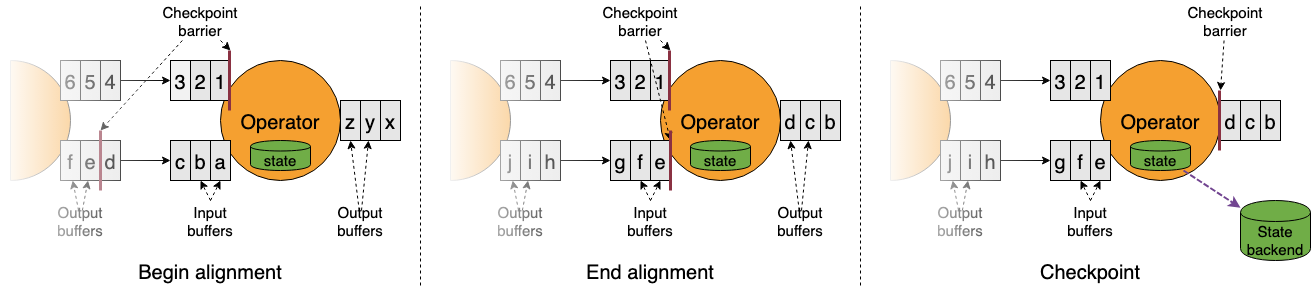
\includegraphics[width=0.88\textwidth]{image/engine/flink_checkpoint_opeartor.png}
  \caption{Barrier alignment at a join operator with two input streams: the operator buffers records from the faster stream until the barrier arrives from the slower stream.}
  \label{fig:flink-checkpoint-operator}
\end{figure}

On failure, all operators roll back to the last complete checkpoint and resume from the
corresponding source offsets.
Combined with a two-phase commit (2PC) sink connector, this delivers
\textbf{exactly-once semantics end-to-end} — no record is lost, no record is duplicated.

\subsubsection{State Storage}

Flink maintains keyed state in pluggable \textbf{state backends}:

\begin{itemize}
  \item \textbf{HashMapStateBackend} — state lives in the JVM heap as Java hash maps.
        Fastest for small-to-medium state; snapshots are serialised and written to the checkpoint store
        (HDFS, S3, GCS) during checkpoint.
        Subject to GC pauses if state grows large.
  \item \textbf{EmbeddedRocksDBStateBackend} — state is stored on local SSD using the RocksDB
        embedded key-value store (native C++ library accessed via JNI).
        Supports state sizes many times larger than available JVM heap with no GC impact.
        Snapshots are uploaded \emph{incrementally} — only changed state is transferred,
        dramatically reducing checkpoint duration for large-state applications.
        Slightly higher per-record read/write latency compared to in-memory, due to disk I/O.
\end{itemize}

\subsubsection{Fault Tolerance}

\begin{itemize}
  \item \textbf{Task failure} — the JobManager restarts the failed task (or the full job, depending on the
        configured restart strategy) and restores its state from the most recent completed checkpoint.
        The source is rewound to the corresponding committed offset, guaranteeing no data loss.
  \item \textbf{JobManager failure} — with high-availability mode enabled
        (backed by ZooKeeper or Kubernetes leader election),
        a standby JobManager takes over immediately without requiring a full job restart.
  \item \textbf{Exactly-once end-to-end} — Flink's checkpoint barriers coordinate with
        transactional sinks (e.g.\ Kafka transactions, JDBC idempotent writes) via a two-phase commit protocol.
        The sink pre-commits data during the checkpoint barrier phase and finalises
        (commits) only after the JobManager declares the checkpoint complete.
\end{itemize}

\subsubsection{Pros and Cons}

\begin{itemize}
  \item[\textbf{+}] True record-at-a-time streaming with sub-millisecond end-to-end latency achievable.
  \item[\textbf{+}] First-class event-time and watermark support — correct handling of late and out-of-order events without application-level workarounds.
  \item[\textbf{+}] Rich stateful operator suite: time-window aggregations, keyed state, complex event processing (CEP), pattern matching, table joins.
  \item[\textbf{+}] Native exactly-once semantics via Chandy-Lamport checkpointing + 2PC sinks.
  \item[\textbf{+}] RocksDB state backend enables very large state (TB-scale) with no JVM GC impact.
  \item[\textbf{--}] Steeper learning curve: JobManager/TaskManager tuning, state backend selection, watermark strategy configuration.
  \item[\textbf{--}] Smaller ecosystem than Spark — fewer connectors, less community tooling, and narrower cloud-managed offering availability.
  \item[\textbf{--}] PyFlink (Python API) lags behind the Java/Scala API in features and performance; some advanced operators require dropping to Java.
\end{itemize}

\subsubsection{Suitable Applications}

\begin{itemize}
  \item Real-time fraud detection and alerting requiring sub-second latency and stateful CEP.
  \item Financial trading systems where exactly-once guarantees are non-negotiable.
  \item IoT telemetry ingestion with high-cardinality keys and out-of-order event-time windows.
  \item Streaming ETL pipelines (e.g.\ Kafka → Flink → Snowflake) where low latency and reliable delivery to the warehouse are required.
  \item Not ideal for ad-hoc exploratory batch analytics or teams already heavily invested in the Spark ecosystem who do not need sub-second latency.
\end{itemize}
